%!TEX root = tesi.tex
\chapter{Background}
\label{ch:background}

Before describing our approach, we give a brief introduction of some of the methods and concepts that are needed to understand our  work. Specifically, we first shortly describe the network technologies required to understand the aim of this project; next, we give an introduction about machine learning and its applications. 

\section{Software-Defined Networking}
Software-Defined Networking (SDN) is paradigm that promises to break networks' vertical integration of control and data plane, separating the network's control logic from the underlying routers and switches, promoting (logical)  centralization  of  network  control,  and  introducing  the ability  to  program  the  network.  The  separation  of  concerns introduced   between   the   definition   of   network   policies,   their implementation  in  switching  hardware,  and  the  forwarding  of traffic, is key to the desired flexibility: by breaking the network control  problem  into  tractable  pieces,  SDN  makes  it  easier  to create and introduce new abstractions in networking, simplifying network  management  and  facilitating  network  evolution~\cite{kreutz2015software}. SDN is loosely built on four principles:
\begin{enumerate}
\item separate control and data planes: network devices are left responsible only of packet forwarding
\item generalized (or flow-based) forwarding: packets are forwarded by looking to a set of fields instead of only the destination, introducing greater flexibility~\cite{mckeown2008openflow}
\item external control logic: the control logic is moved to an external entity called SDN controller or Network Operating System (NOS), that is a software platform that provides abstractions to facilitate the programming of forwarding devices
\item programmable network: software running on top of the NOS allows to program the network; this is considered the main value of SDN.
\end{enumerate}
SDN has successfully opened the way towards a next generation networking, creating an innovative research
and  development  environment,  promoting  advances  in  switch  and  controller platform design,  evolution of performance  of  devices  and  architectures, security and dependability~\cite{sdnsurvey}.

\section{Knowledge-Defined Networking}
Knowledge-defined networking (KDN)~\cite{mestres2017knowledge} is a new paradigm that promotes the application of Artificial Intelligence (AI) to control and operate networks thanks to the rise of SDN. SDN provides a centralized control plane, a logical single point with knowledge of the network; moreover, current network devices have improved computing capabilities, which allow them to perform monitoring operations commonly referred to as network telemetry~\cite{kim2015band}. Information provided by network telemetry are usually provided to a centralized Network Analytics (NA) platform~\cite{clemm2015dna}, that combined with SDN can bring to light the Knowledge Plane proposed in~\cite{clark2003knowledge}. Knowledge-Defined Networking is the paradigm resulting from the combination of these tools, specifically Software Defined Networking, Network Analytics and Knowledge Plane. In the KDN paradigm, the knowledge plane has a rich view of the network; this view is transformed into knowledge via Machine Learning (ML) and used to make decisions. The ultimate goal of KDN is to combined SDN, Network Analytics  and Machine Learning to provide automated network control.
%
\section{Routing}
In networking, routing is the process of selecting a path in or between networks. Routing directs network packets from their source toward their destination through intermediate network nodes by specific packet forwarding mechanisms. Forwarding is performed on the basis of routing tables, which maintain a record of the routes to various network destinations. Thus, constructing routing tables, is very important for efficient routing. Dynamic routing constructs routing tables automatically thanks to the information carried by the routing protocols, that are usually classified in \textit{distance vector} and \textit{link-state} algorithms.

\paragraph{BGP} (Border Gateway Protocol) is a protocol designed to exchange routing and reachability information among or within Autonomous Systems (AS). An average AS is made by about 500 point of presences, and together ASes glue the Internet together. When used to route packets across ASes of the same Internet Service Provider (ISP) BGP is also referred to as Internal BGP, or iBGP. In contrast, to route across ASes BGP uses other ``External BGP`` protocols, or eBGP. BGP is typically used by ISPs to establish routing between one another, or in large private networks to join a number of large networks. Routing informations are exchanged between neighbor routers (or peers); to communicate, these peers often require a manual configuration.

\paragraph{OSPF} is a link-state algorithm and it requires IP. OSPF falls in the family of iBGP and it is widely adopted in large networks.  The majority of ISP use a version of Open Shortest Path First (OSPF). It works thanks to a map of the network, built by gathering link state information from available routers. The maps is used to compute the shortest-path tree for each route using a method based on Dijkstra's algorithm~\cite{dijkstra1959note}. The OSPF routing policies are dictated by link metrics associated with each routing interface, typically the interface speed.

\section{Machine Learning}
Machine learning is a field of computer science that studies the ability of making computers learn without explicitly programming them~\cite{5392560}. In machine learning there are three main approaches: supervised learning, unsupervised learning and reinforcement learning. Supervised learning is used to classify labeled data, where the label is a sort of supervisor describing the class of an observation. In unsupervised learning, data is unlabeled and the goal is to find the hidden relation among data records. Reinforcement learning is learning what actions to apply so as to maximize a numerical reward signal without being told which actions to take but instead discovering which yield the most reward by trying them \cite{Sutton98reinforcementlearning}. Among the several branches of machine learning, neural networks and in particular deep learning, have recently attracted a lot of attentions.

\subsection{Deep Learning}
Teaching a computer to solve tasks that are hard to describe formally (e.g., speech recognition or routing) is challenging; the solution is to allow computers to learn from experience and understand the world in terms of a hierarchy of concepts, with each concept defined through its relation to simpler concepts. The hierarchy of concepts enables the computer to learn complicated concepts by building them out of simpler ones. If we draw a graph showing how these concepts are built on top of each other, the graph is deep, that is, it has many layers~\cite{Goodfellow-et-al-2016}. Deep learning can be described as the set of machine learning techniques that concatenate multiple layers of processing units (typically non-linear), for feature extraction and transformation~\cite{deep_learning_heterogeneus}. 

The first working deep learning algorithm was a multilayer perceptrons developed by Ivakhnenko et al.~\cite{ivakhnenko1973cybernetic}. Later on, new techniques including Convolutional Neural Networks (CNNs) and Recurrent Neural Networks (RNNs) were developed; these techniques dramatically increased Artificial Intelligence performance in tasks such as image recognition. More recently, deep learning has been used to successfully play games, see AlphaGo~\cite{alphago}.

\subsection{LSTM}
Long Short-Term Memory (LSTM) is a further development of Recurrent Neural Networks (RNNs). They were developed by Hochreiter and Schmidhuber in 1997 and have been further improved ever since~\cite{Greff2016}. The major flaw of a traditional neural network that RNN improves, is that it does not capture the relation between the input it currently looks at and the previous training example. Such relation is, however, crucial for example to develop a (human) language model. Making predictions about a subsequent word strongly depends on the semantic of preceding words. In practice, RNNs are also not scalable when trying to model long-term dependencies. 
This is due to numerical problems commonly referred to as the \textit{vanishing/exploding gradient}~\cite{bengio1994learning} when weight updates are back-propagated through the time steps. During the backpropagation	phase, the weights of the network are updated according to the computed gradients; the magnitude of gradients is affected by the weights and the activation functions.
If either of these factors is smaller than one, then the gradients may vanish in time when propagating to the first layers of the network; similarly, if larger than one, then exploding might happen. LSTMs overcome this problem and enables capturing long-term temporal dependencies among the input elements. LSTMs are considered state-of-the-art in numerous sequential prediction tasks such as Speech Recognition, Handwriting Recognition, Language Translation and many others.

The novelty of LSTMs compared to conventional RNNs is the introduction of the \textit{LSTM cell}. Figure~\ref{fig:lstm} gives an overview over such a cell that is repeated three times, each receiving the current input as well as the output of the previous cell. For instance, the prediction $h_{t+1}$ (through feed-forward) is based on the corresponding input $x_{t+1}$ as well as on the output of the previous cell. The LSTM cell is responsible for maintaining and updating a state that keeps track of the input that has been processed over time. Which information precisely should be kept and which overwritten is decided during the training phase of the RNN. Each cell has associated weights that are updated during each backward pass such that the cell keeps the information that optimizes predictions. The major advantage of introducing this cell is that the \textit{Back-propagation Through Time} does not need to flow through numerous activation gates between the hidden layers. The transfer from cell to cell only flows through pointwise multiplications and additions. This way the numerical problems of RNNs are avoided.

\begin{figure}
\centering
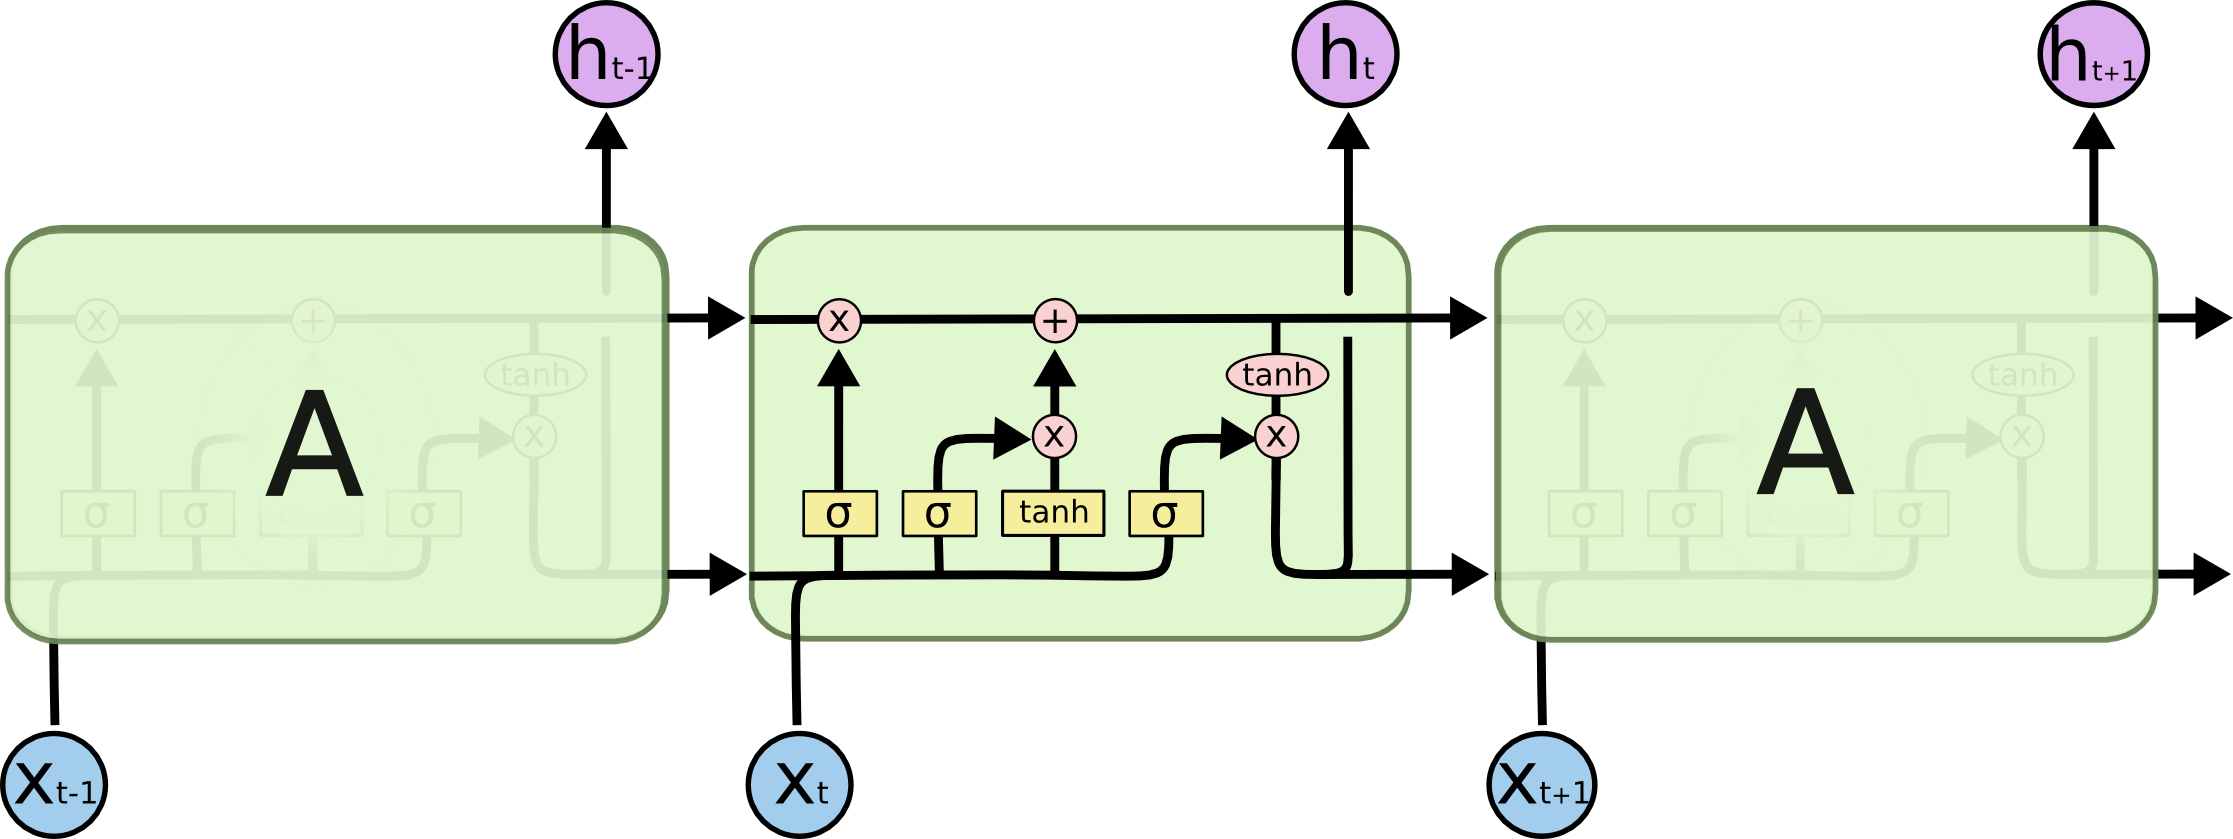
\includegraphics[width=0.9\textwidth]{img/lstm}
\caption{LSTM cell overview.\protect\footnotemark}
\label{fig:lstm}
\end{figure}
\footnotetext{Taken from colah's blog:~\url{http://colah.github.io/posts/2015-08-Understanding-LSTMs/}}

